%*****************************************
\chapter{Literature Review}

\section{Deep-learning based runway segmentation}

In \cite{akbar_runway_2019}, the authors give a broad literature review of the
prior work on runway segmentation using traditional and deep-learning methods.
They break down the traditional methods into two categories: template-based and
feature-based approaches, the former compares a template image to the actual one
pixel-by-pixel, and the latter uses edges, corners, texture, and others to
detect and localize the runway. They find that most works that use deep-learning
methods are focused on airport detection, and not runway segmentation,
highlighting the paper's relevance.

They then propose a two-module pipeline, where the first module is responsible
for detecting runway presence and the second module is responsible for
localizing it. For the detection module, they fine-tune a pre-trained ResNet50 model, achieving an accuracy of 97\%. And for the localization module, they experiment with three approaches: Hough transform, line segment detector, and a CNN, 
achieving a 0.8 mean IoU (Intersection-over-Union) score.

The study shows that deep-learning methods are a valid and effective pathway to
runway detection and segmentation, but there are significant shortfalls with it
for practical vision-based landing systems. The top-down perspective from the
satellite dataset images (\emph{"Remote Sensing Image Scene Classification"} \cite{cheng_remote_2017}) is unrealistic for fixed-wing aerial vehicles' approach and landing, because the onboard system needs to detect and segment runways from the perspective of the aircraft. Secondly, there are no discussions on dataset diversity such as adverse weather and lighting conditions and the performance of the pipeline in those cases.

In \cite{chen_bars_2023}, the authors note the lack of large-scale, publicly available datasets for the field of runway segmentation. Trying to alleviate this problem, they propose \emph{"BARS: A Benchmark for Airport Runway Segmentation"}, a 10,256-image labeled runway dataset, with images collected from X-Plane, a FAA-certified flight simulator. The images were collected from several simulated flights under different weather conditions and at different times, across 40 airports, to generate a diverse dataset far more suitable for the task of vision-based landing than the one used in \cite{akbar_runway_2019}.

To test the efficacy of this new dataset, they experiment with several segmentation methods (e.g., Mask R-CNN, YOLACT, SOLO) and report the trained models' performance, which have a wide range of reported precisions (AP50 of 90.98\% for the best performing one and 62.18\% for the worst performing one).

At the same time, using a simulator for generating synthetic images limits
scenario diversity (e.g., it is not possible to create scenarios in airports that
are not included in the simulator). Also, because it is a closed-source
simulator, it is not easy or accessible for other researchers to expand on this
dataset by adding more diverse and unseen scenarios. And the manual labeling
process using LabelMe \cite{mit_labelme_nodate} also increases the cost of
reproducing or expanding the dataset. Another problem of the work is that the
authors decided to publish their work on Baidu, which prevents access to the
full dataset without installing a third-party program on the computer.

The way the authors decided to test \emph{BARS} experimentally highlights a situation that is similar to the problem encountered by Nobel-winning economist Eugene Fama in his work on Efficient Markets \cite{fama_efficient_1970}: the joint hypothesis problem. The joint hypothesis problem is the fact that all tests of market efficiency are simultaneously tests of market efficiency and the asset pricing model that defines expected returns. Therefore, anomalous market returns might be due to market inefficiency, an inaccurate model, or both. 

\phantomsection
\label{sec:joint_hypothesis}
Similarly, when proposing new datasets, one has to always be mindful that
empirical tests of training models on these new datasets \emph{are always a joint test of dataset quality and model performance}. A model's poor performance might indicate deficiencies in the dataset (e.g., lack of diversity, poor annotation quality, or unrealistic synthetic images), a reflection of the model's limitations in handling a more realistic dataset with more complex tasks, or both. On the other hand, if a model performs really well, it doesn't automatically prove that the dataset is good. It could mean the dataset simply matches the model's strengths, without really testing how well it would work on real-world images.

In \cite{chen_image-based_2024}, the authors propose \emph{"ERFE: efficient
runway feature extractor"}, a runway detection model that is able to extract
semantic segmentation and feature lines. Also highlighting the difficulties of
runway datasets, the authors propose a new synthetic image dataset
\emph{"FS2020"}, using images from Microsoft's Flight Simulator 2020. They did have access to BARS but argued that the images from X-Plane were unrealistic, especially in regards to ground texture and lighting conditions. Their proposed dataset contains 5,587 high-resolution (1920x1080) images, sampled from different runways, airplane positions, and lighting and weather conditions.

After image collection, the authors used the LabelMe toolbox to provide two types of annotation for each image: segmentation masks and feature lines with 6 categories (left edge, right edge, center line, aiming point front, threshold rear, and PAPI lights).

The authors highlight the need for fast and accurate inference in the context of a fast-moving airplane. Thus, they chose to build a deep-learning model based on MobilenetV3, a convolutional neural network designed for mobile phone CPUs. They claim that their trained network has the capacity of processing 200 high-resolution images per second.

Their work excels in demonstrating the feasibility of an onboard runway
segmentation system, and their FS2020 dataset is a rich contribution to the
field, especially as it is accompanied by segmentation and feature lines labels.
At the same time, it is a smaller dataset when compared to BARS, and because it
is also based on a closed-source simulator, it has the same trade-offs
associated with it. The authors also didn't compare their model's performance when
trained with another dataset like BARS, which would make it easier to understand
how well their dataset generalizes compared to others. Without this comparison,
it is unclear whether their model performs well because of the dataset's quality
or simply because the dataset aligns well with the model's training conditions.
On the other hand, they hosted the dataset on Kaggle, a widely used platform for hosting public datasets.

In \cite{ducoffe_lard_2023}, the authors still highlight the lack of open-source datasets of aerial images of runways and present, the \emph{"LARD: Landing Approach Runway Detection"} dataset, a novel 17,000-image dataset alongside an image generator. They use Google Earth Studio, positioning a camera inside the studio in the perspective of an airplane nose pointing to the runway. They publicly shared their generator scripts that automatically output labeled images without the need for human intervention. Alongside the generated synthetic data, they manually labeled real videos from airplanes landing.

Their method has considerable advantages over simulator-based ones: it is
possible to reproduce and generate new images for virtually free, as Google
Earth Studio is a closed-source but free tool, with lower need for manual
labeling. On the other hand, the images are less realistic than the simulator-based ones, as the ground texture is worse and it lacks different weather conditions, and night view is simulated by a simple reduction in ambient brightness.

The authors don't train any detection or segmentation models based on the
\emph{LARD} dataset in the paper, but \cite{li_yolo-rwy_2024} did introduce
YOLO-RWY, a YOLO-based \cite{redmon_you_2016} deep-learning model, and trained it using LARD, reporting that it has \emph{"strong generalization and real-time capabilities"} \cite{li_yolo-rwy_2024}. The authors highlight how the limited nighttime and adverse weather samples in LARD may affect performance in extreme conditions, and they did include a data augmentation step in their training pipeline.

In \cite{wang_valnet_2024}, the authors built VALNet, a model based on YOLO that uses band-pass filters to be able to handle large-scale changes and input image angle differences in the context of runway segmentation. Among the reviewed papers on runway segmentation models, it is by far the most advanced, with a novel architecture and extensive comparisons to other models, such as YOLOv8 and Mask R-CNN.

The paper also cited the dataset scarcity challenge and proposes a new dataset called \emph{"RLD (Runway Landing Dataset)"}, with 12,239 images with a resolution of 1280x720. The images are sourced from X-Plane, similarly to the already reviewed BARS. The dataset was also manually labeled using LabelMe, and the dataset is also hosted on Baidu. Although it is the largest simulator-based dataset reviewed in this paper, it has the same advantages and disadvantages as previously reviewed simulator-based datasets.

\section{Image generation models}

GANs (generative adversarial networks) were introduced by \cite{goodfellow_generative_2014}, and they consist of two neural networks, the Generator and the Discriminator, engaged in adversarial training. The generator is responsible for creating synthetic images (in the context of image GANs) and the discriminator is responsible for evaluating the authenticity of images. During training, the generator gets better at creating realistic images and the discriminator gets better at differentiating real from synthetic images.

In \cite{cohen_generative_2022}, the authors give a survey on the main issues of GANs and their applications. They show how GANs can be effectively used for data augmentation, and with other GAN architectures such as Semi-supervised GAN (SGAN), there can be a model that outputs labeled images. But GANs suffer from a well-known problem called "mode collapse," where the generator learns to produce only one or a few specific patterns that fool the discriminator, making the range of images generated by the model less diverse.

Diffusion models, introduced in \cite{ho_denoising_2020}, are a generative approach based on iterative denoising. Diffusion models work by progressively adding noise to an image (called the forward process) and then training a network that learns how to remove noise from the image (the reverse process).

\begin{figure}[htbp]
\centering
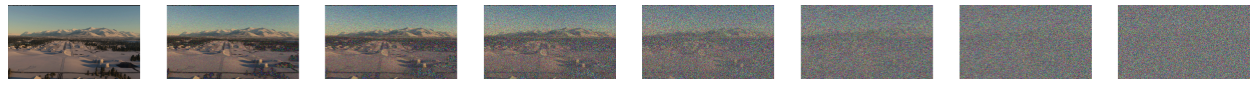
\includegraphics[width=1.2\textwidth]{figures/noise_to_image.png}
\caption{Example of Diffusion forward process adding noise to an image}
\label{fig:noise_to_image}
\end{figure}

The intuition of Diffusion models is that, if a model can be trained to predict
the noise in an image at a \emph{timestep}, we can start at pure noise, then repeatedly call this model and remove the noise from the image, at each step making a less noisy image.

A key architecture used in diffusion models is U-Nets, introduced in \cite{ronneberger_u-net_2015}. The U-Net is composed of two parts: an encoder and a decoder. The encoder transforms the image into a compressed form that retains essential features. This compressed data is called a "latent". The decoder can then operate on this latent and output some data related to the input data. In the original paper, they used the U-Net to extract biomedical segmentation data. In Diffusion models, the U-Net is used as the model that predicts the noise from an image.

\begin{figure}[htbp]
\centering
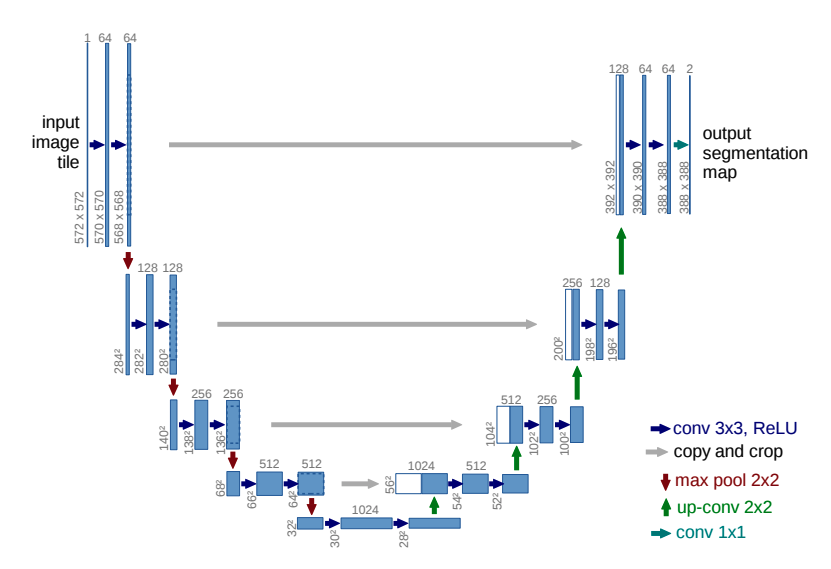
\includegraphics[width=1.0\textwidth]{figures/unet_architecture.png}
\caption{U-Net architecture. Figure from \cite{ronneberger_u-net_2015}}
\label{fig:unet_architecture}
\end{figure}

Although recently diffusion models have emerged as the new state-of-the-art architecture for image generation \cite{yang_diffusion_2024}, they do have disadvantages. Namely, their inference time is slower than that of GANs, they have a higher computational cost, and by themselves, they lack mechanisms for precise editing of the image aside from the text prompt.

This problem of controlling the generated image was tackled by \cite{zhang_adding_2023}, which introduced ControlNet. ControlNet is a neural network that allows spatial conditioning to pre-trained text-to-image models. With it, it is possible to use canny edges, human poses, and segmentation masks to control the final result of the image. This allows greater control over the generation of synthetic images, such as the positioning of a runway in an image or control over the markings and detailed paintings on the runway.

\section{Synthetic datasets built with diffusion models}

In \cite{saragih_using_2024}, the authors cite a similar data scarcity problem in the field of medical images, specifically, gastrointestinal images. To solve this problem, they built a pipeline that used diffusion models to generate labeled gastrointestinal polyp images.

They started by clustering the training images and masks into 20 different clusters, and after that, training a four-channel (3 for RGB and a binary one for the mask) DDPM (Denoising Diffusion Probabilistic Model) for each cluster. The models were trained with a fourth channel so that the model outputs an image and the associated mask along with it, requiring no human labeling. They used the RePaint \cite{lugmayr_repaint_2022} technique to guide the diffusion process so that the polyp was always generated in a specific area of the images, and they also used styling techniques so that the generated images were realistic. 

They compared the diffusion-generated images with GAN model-generated images
and found that the diffusion images were closer to real ones. The study trains
several diffusion models to address the problem of large variation between
images in the dataset, making each model specialize in its cluster. The paper shows promising results that we can augment image datasets with diffusion models, but only low-resolution images were generated (256x256 pixels) and a larger variety of images would require training more independent models.

In \cite{reutov_generating_2023}, the author explored using text-to-image
diffusion models to generate urban traffic images for vehicle detection and
classification. The author used the trained Kandinsky 2.2 model to generate
images using \emph{prompt engineering}. 192 different prompt variants were used to generate 1000 images with different combinations of traffic density, type of vehicle, location, weather condition, time of day, and camera location. The paper shows how far off-the-shelf models are capable of generating realistic images that can be used to train detection algorithms. But it does not compare images generated by different models, and the images have to be manually labeled. 

In \cite{voetman_big_2023}, the authors studied the effectiveness of fine-tuning
a pre-trained Stable Diffusion model for the purpose of generating datasets,
applied to apple detection in apple orchards. They separated their baseline
dataset into two datasets: green apples and red apples. After that, they
fine-tuned two Stable Diffusion models with DreamBooth and then generated a
whole dataset. They used a trained apple detection model for baseline image
annotations and then manually refined these annotations. To experimentally test
the effectiveness of their datasets, they trained multiple YOLO \cite{redmon_you_2016} object detectors on the baseline and synthetic datasets and compared the results. In their study, object detectors performed similarly when trained on their synthetic dataset and when trained on real image datasets. Their approach shows promising results in dataset generation with Stable Diffusion, although there is a lack of diversity (e.g., weather conditions, lighting conditions, different backgrounds, etc.) in both the baseline dataset that makes it easier to generate a synthetic dataset that is similar to the original.

\section{Evaluation of Synthetic Data}

Across the previously mentioned works, two types of evaluation were common: theoretical similarity and experimental performance. Theoretical similarity was assessed using metrics such as FID (Fréchet Inception Distance) \cite{heusel_gans_2017} and SSIM (Structural Similarity Index) \cite{wang_image_2004}, which measure the similarity between two images. Theoretical similarity was used to evaluate the synthetic datasets in \cite{saragih_using_2024}. Experimental performance, on the other hand, is about training a model on the synthetic dataset and comparing the results. Experimental performance was used in all runway segmentation papers, except for LARD, and also in \cite{reutov_generating_2023, voetman_big_2023}.

Both forms of testing are valid and have their trade-offs. Theoretical similarity is faster and easier to measure but heavily depends on what images are included in the test. And if a dataset contains very different image structures than the original, even if they are high-quality, the FID/SSIM give worse values. On the other hand, experimental performance tests the dataset in a realistic setting, evaluating how it will be used by other researchers, but suffers from the joint dataset-model problem covered previously.
